\exercisetitle{
Una línea de transmisión sin perdidas de longitud $0.3\lambda$ termina en una impedancia de carga, $Z_L$. Encontrar
el coeficiente de reflexión en la carga, el SWR de la linea y la impedancia de entrada de la linea. $(Z_0=75
\Omega, Z_L = 40 + j20 \Omega)$.
}
Para calcular primeramente el coeficiente de reflexión, situaremos en la carta de Smith el punto $z = \frac{40}{75} + \frac{20}{75}j \Omega$, marcado con un '1' en al gráfica. Donde observando el ángulo y la fase de este punto, obtenemos:
\[ \Gamma_L = 0.34e^{j2.45} \]

Para calcular el SWR haremos:
\swr{ \approx 2}

Para calcular la impedancia a la entrada moveremos el punto '1' $0.3 \lambda$ hacia el generador, punto '2' y observaremos que lineas corta. En este caso:
$z_i = 0.94 + 0.7i$ que al denormalizar quedará como: $Z_{in} = 67.5 + 52.5j$.

\begin{figure}[h]
  \centering
  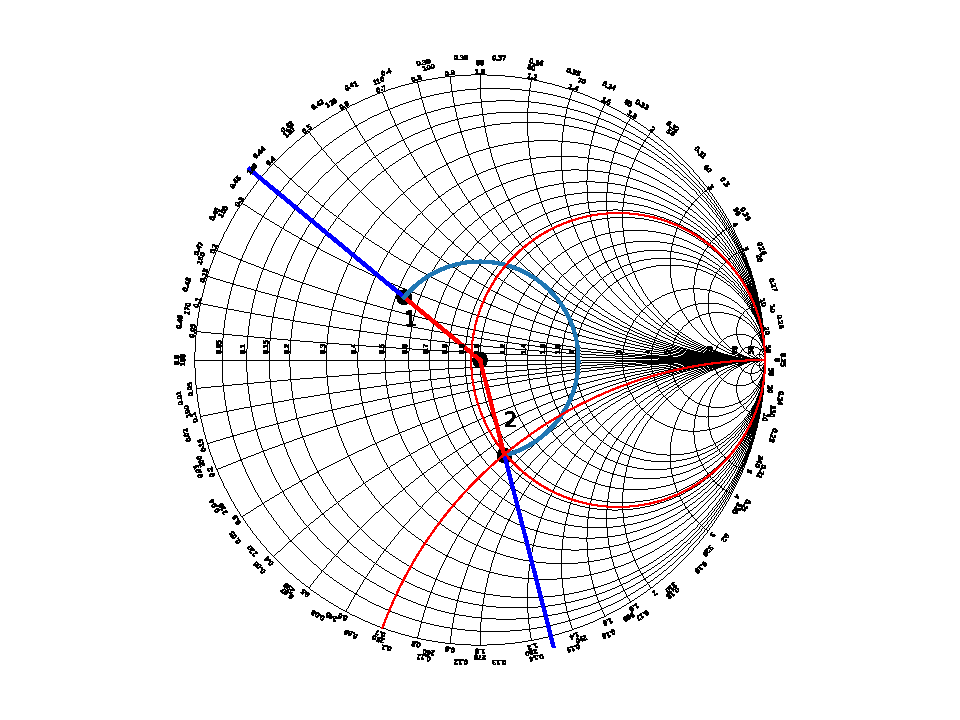
\includegraphics[scale = 0.85]{ej2/images/out.pdf}
  \caption{Moviendo el punto $0.3 \lambda$}
  \label{ej2smith}
\end{figure}
